
%%% Local Variables: 
%%% mode: latex
%%% TeX-master: t
%%% End: 

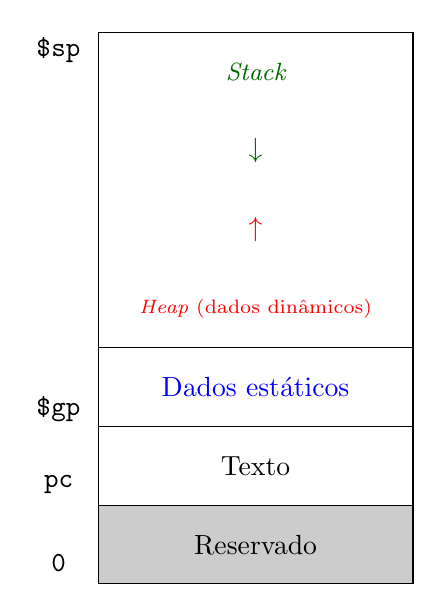
\begin{tikzpicture}
  \node[rectangle,draw,minimum width=4cm,minimum
  height=1cm,fill=gray!40]  (reserved) {Reservado};
  \node[rectangle,draw,minimum width=4cm,minimum
  height=1cm] (text) [above of=reserved] {Texto};
  \node[rectangle,draw,minimum width=4cm,minimum
  height=1cm] (static) [above of=text] {\color{blue}Dados estáticos};
  \node (heap) [above of=static] {\scriptsize \color{red}{\em Heap} (dados
    dinâmicos)};
  \node (up) [above of=heap] {\color{red}$\uparrow$};
  \node (down) [above of=up] {\color{green!40!black}$\downarrow$};
  \node (stack) [above of=down] {\small {\color{green!40!black}\em Stack}};
  \node[rectangle,draw,minimum width=4cm,minimum height=6cm,yshift=5mm] (rect) [above of=static] {};

  \node [left of=reserved,xshift=-15mm,anchor=north] {\tt 0};
  \node [left of=text,xshift=-15mm,anchor=north] {\tt pc};
  \node [left of=static,xshift=-15mm,anchor=north] {\tt \$gp};
  \node [left of=stack,xshift=-15mm,anchor=south] {\tt \$sp};

\end{tikzpicture}